% Figure snippets — embedded inline by main.tex
\begin{figure}[t]
  \centering
  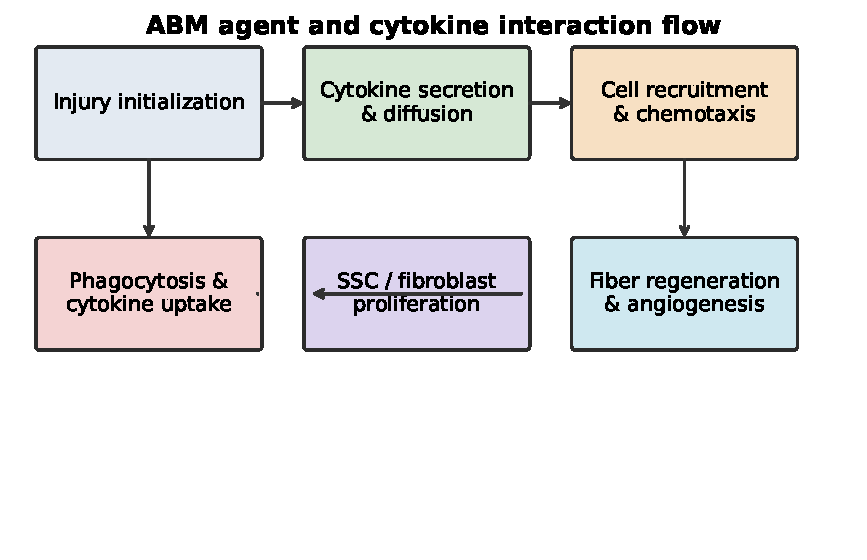
\includegraphics[width=0.95\linewidth]{figures/fig_overview.pdf}
  \caption{Overview of the agent-based model. Cells, cytokines, and the extracellular matrix interact through recruitment, chemotaxis, phagocytosis, secretion, and binding, with cytokine diffusion recalculated as local collagen density changes.}
  \label{fig:overview}
\end{figure}

\begin{figure}[t]
  \centering
  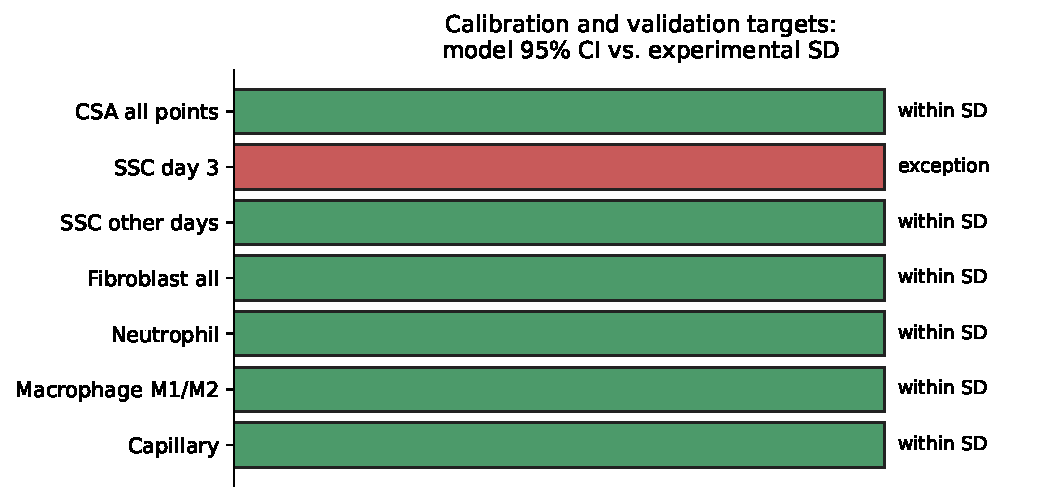
\includegraphics[width=0.90\linewidth]{figures/fig_calibration.pdf}
  \caption{Calibration and held-out validation outcomes. Green bars indicate targets whose model 95\% confidence interval falls within the experimental standard deviation; the single exception (satellite stem cell count at day 3) is shown in red.}
  \label{fig:calibration}
\end{figure}

\begin{figure}[t]
  \centering
  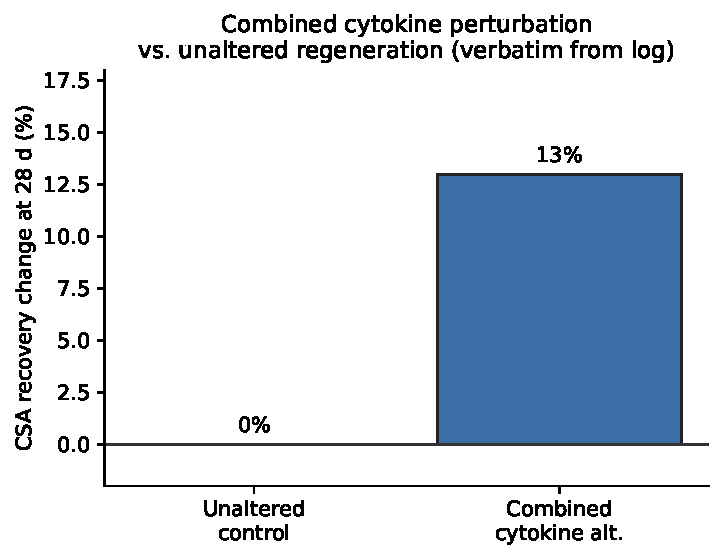
\includegraphics[width=0.70\linewidth]{figures/fig_perturbation.pdf}
  \caption{CSA recovery at 28 days: combined cytokine perturbation relative to unaltered regeneration. The 13\% improvement is taken verbatim from the experimental log; no other perturbation magnitudes are shown numerically.}
  \label{fig:perturbation}
\end{figure}

\begin{figure}[t]
  \centering
  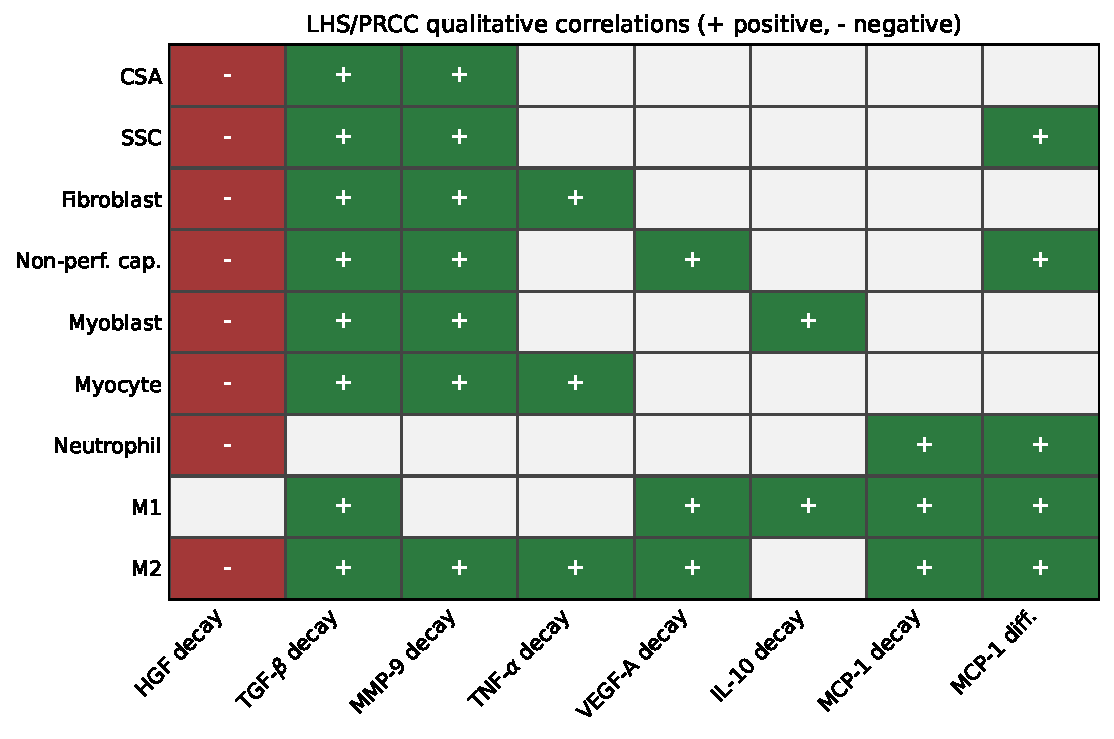
\includegraphics[width=0.95\linewidth]{figures/fig_sensitivity.pdf}
  \caption{Qualitative LHS/PRCC sensitivity matrix compiled from the supplemental sensitivity analysis description. ``+'' and ``-'' cells indicate statistically significant positive and negative correlations between cytokine decay or diffusion parameters and model outputs.}
  \label{fig:sensitivity}
\end{figure}
